\documentclass{article}

\usepackage[utf8]{inputenc}
\usepackage[top=2cm, left=2cm, right=2cm, bottom=2cm]{geometry}
\usepackage{subfig}
\usepackage{graphicx}

\title{Homework 8 - Image mining \\
        \vspace{5px} \large UTFPR - CPGEI - Data Mining \\
        Prof. Dr. Heitor Silvério Lopes}
\author{Vinícius Couto Tasso}
\date{November 2019}

\begin{document}

\maketitle

This work presents two different approaches to the task of feature extraction on images for classification. The first method consists of using implementations of well-known image filters on Weka\footnote{Weka is a collection of machine learning algorithms for data mining tasks written in Java.}, such as:

\begin{itemize}
    \item Gabor Filter - A commonly image filter used filter in computer vision, capable of extracting texture features that are invariant to rotation;
    \item RGB Color Histogram Filter - A very basic image filter that consists in three histograms (red, green and blue), each of which has 32 bins. Each bin contains a count of pixels that fall into its respective color range;
    \item PHOG Filter - Pyramid Histogram of Oriented Gradients, a very widely used image filter on literature, encodes information about the orientations of intensity gradients across an image.
\end{itemize}

The second method makes use of pre-trained convolutional neural networks, available on Orange\footnote{Orange is a component-based visual programming software package for data visualization, machine learning, data mining, and data analysis written in Python.}, to generate features vectors. 

The provided dataset contains two groups: Group A is made of 11 vehicle classes, each with 10 images (110 images). Group B contains 9 vehicle classes with 200 images each (1800 images). Table \ref{tab:dataset_overview} presents an overview of the dataset.

\begin{table}[h]
    \centering
    \begin{tabular}{c|c}
         \textbf{Group A} & \textbf{Group B} \\ \hline
        Airplane & \\
        Bicycle & Bicycle \\
        Truck & Truck \\
        Articulated truck & Articulated truck \\
        & Pickup truck \\
        Motorcycle & Motorcycle \\
        Bus & Bus \\
        Pedestrian & Pedestrian \\
        Tractor & \\
        Train & \\
        Van & Van \\
    \end{tabular}
    \caption{Overview of the vehicle classes contained in each group of the dataset}
    \label{tab:dataset_overview}
\end{table}

\section*{Weka}

Experiments were conducted with features generated by filters individually and with features from all three filters. After the generation of features, the classification was done using the C4.5 decision tree algorithm (called J48 on Weka implementation), with the baseline being established by OneR. The results are shown on Table \ref{tab:weka_table}.

\begin{table}[hbtp]
    \centering
    \begin{tabular}{c|c|c|c|c}
        \textbf{Filters} & \multicolumn{2}{c|}{\textbf{Group A}} & \multicolumn{2}{c}{\textbf{Group B}} \\ \hline
         & \textbf{OneR} & \textbf{J48} & \textbf{OneR} & \textbf{J48}  \\
         \textbf{Gabor} & \textbf{0.155} & 0.200 & 0.201 & 0.227 \\
         \textbf{RGB} & 0.145 & \textbf{0.209} & 0.206 & \textbf{0.374} \\
         \textbf{PHOG} & 0.118 & 0.164 & \textbf{0.217} & 0.323 \\
         \textbf{Gabor + RGB + PHOG} & 0.100 & 0.191 & 0.201 & 0.368 \\
     \end{tabular}
    \caption{Comparison of TPR rate for different combinations of filters for each group of the dataset.}
    \label{tab:weka_table}
\end{table}


Results show that in both cases the RGB Color Histogram Filter performed the best. This means that, for this problem, color is a better feature for classification than texture and border, despite being the simplest approach. It is very clear as well that this is not a problem easily solvable by just applying conventional image filters since even the best results are far from being considered a robust classification.

It is important to note that, besides classes and size differences, Group A and Group B are very distinct: most images on Group A are high resolution and apparently were taken very close to the object (by a person, for example), with the exception being airplane photos. Group B is made solely of images taken by what seems to be traffic surveillance cameras, meaning that they are usually relatively far and above the object, and the pictures are low resolution.

Table \ref{tab:best_worst} presents the two best and worst classes (based on TPR rate) classified by J48 using RGB Histogram filter.


\begin{table}[htbp]
    \centering
    \begin{tabular}{c|c|c|c|c}
         \textbf{Criteria} & \multicolumn{2}{c|}{\textbf{Group A}} & \multicolumn{2}{c|}{\textbf{Group B}} \\ \hline
         \textbf{Best TPR Classes} & Airplane (0.700) & Pedestrian (0.300) & Motorcycle (0.480) & Bicycle (0.465) \\
         \textbf{Worst TPR Classes} & Motorcycle (0)  & Train (0) & Pickup truck (0.275) & Van (0.285) \\
    \end{tabular}
    \caption{Two Best and worst classification TPR rate for each group.}
    \label{tab:best_worst}
\end{table}

Further analysis of data provides some insights into why that might be the case. On Group A, it is very evident that the Airplane class is the easiest to identify only with colors: the background in most cases is blueish and the airplanes are white or gray. 
Pedestrians probably had better accuracy than other classes because, since they don't occupy a very large portion of the image, the street does and, therefore, the gray color ends up being very prominent on these images.
Motorcycles were frequently miss classified as bicycles and trains as motorcycles, interestingly. 

Group B is a much more homogeneous group of images, given the similarity between each image. Despite that being the case, two classes are very distinct from all other vehicle classes in both color and shape: Motorcycle and Bicycle. Not surprisingly, these were the two best-classified classes. Pedestrians are very distinct from the other vehicles as well, but they were often miss classified as bicycles, lowering the class TPR rate by a considerable amount.

In regards to information comprehensibility versus classification accuracy, given the complexity of the output of the C4.5 algorithm when compared to OneR, if the goal is to understand what kind of feature determines the class of a given image, OneR is a better option here, since neither of the approaches was able to obtain satisfactory results.

In conclusion, it is clear that the fact that Group A has high-quality images doesn't make up for the fact that it has a very limited amount of samples,  as well as some images that are very different from each other, besides belonging to the same class, which only makes it harder to define a homogeneous class of images for the classification algorithm.


\section*{Orange}

In opposition to the experiments performed within Weka, this section is focused on extracting features with deep neural networks trained on a different dataset. The neural net of choice is Inception-v3, trained on the ImageNet dataset\footnote{ImageNet is a dataset composed of approximately 14 million images of 1000 different classes.}, capable of extracting 2048 different features from an image. All the training and evaluation of this section were performed using the Orange software.

Table \ref{tab:inception_baseline} presents the results of classification of the default neural network implementation on Orange, with the features extracted by Inception as input and tenfold stratified cross-validation. The results show that, compared to the filters applied in the previous experiment, this is a much more robust approach with far superior results.

\begin{table}[htbp]
    \centering
    \begin{tabular}{c|c|c|c}
         & \textbf{AUC} & \textbf{Accuracy} & \textbf{F1 score}  \\ \hline
         \textbf{Group A} & 0.987 & 0.918 & 0.918 \\
         \textbf{Group B} & 0.962 & 0.736 & 0.734 \\
    \end{tabular}
    \caption{Classification results using a neural network trained on features extracted by Inception.}
    \label{tab:inception_baseline}
\end{table}

As previously mentioned, Group B is a much more homogeneous set of images, making it much harder to distinguish different classes, since they are all similar to an extent.
Figures \ref{fig:conf_matrix_a} and \ref{fig:conf_matrix_b} show more details on classification results of both image groups. The rows highlighted in green are the percentage of correctly classified instances of a given class, whereas the red rows are the percentage of miss classified instances.

\begin{figure}[htbp]
    \centering
    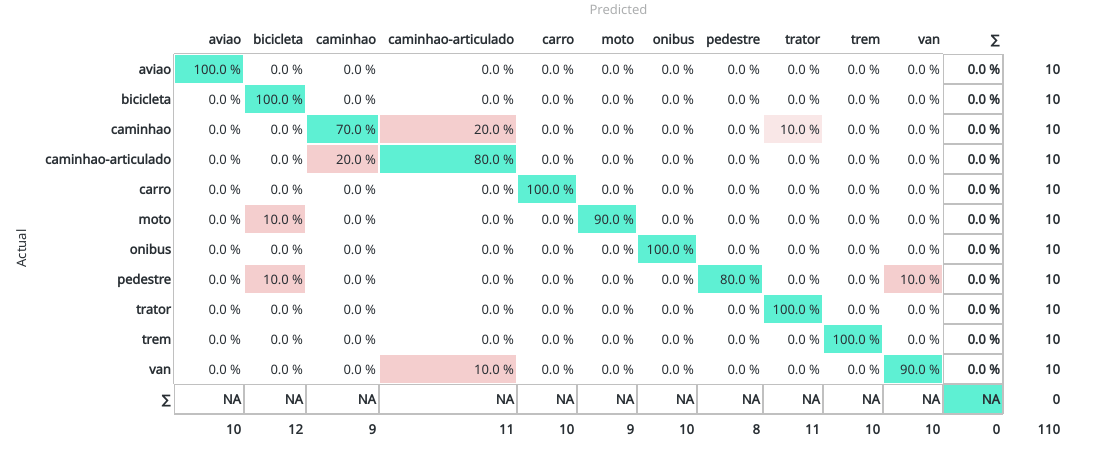
\includegraphics[scale=0.52]{cm_grpa.png}
    \caption{Confusion matrix of Group A images classification.}
    \label{fig:conf_matrix_a}
\end{figure}

\begin{figure}[htbp]
    \centering
    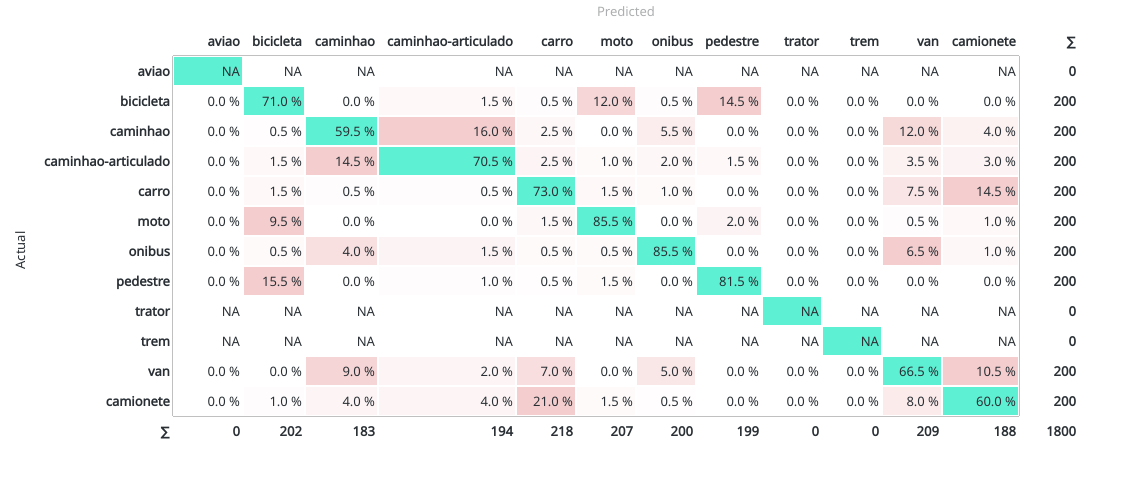
\includegraphics[scale=0.52]{cm_grpb.png}
    \caption{Confusion matrix of Group B images classification.}
    \label{fig:conf_matrix_b}
\end{figure}

The next experiment is on transfer learning and the objective is to evaluate the performance of a neural network trained on a group of images predicting images belonging to the other group.

\begin{table}[htbp]
    \centering
    \begin{tabular}{c|c|c|c|c}
         \textbf{Train} & \textbf{Predict} & \textbf{AUC} & \textbf{Accuracy} & \textbf{F1 score}  \\ \hline
         \textbf{Group A} & \textbf{Group B} & 0.709 & 0.248 & 0.239 \\
         \textbf{Group B} & \textbf{Group A} & 0.792 & 0.409 & 0.347 \\
    \end{tabular}
    \caption{Results of a network trained on one group of images put to make predictions on the other image group.}
    \label{tab:transfer_learning}
\end{table}

As expected, the network that trained on the ``easier'' portion of the dataset, which is also the one with the least amount of samples, had a harder time when compared to the network that switched to a less difficult classification task.
\pagebreak
It is interesting to note that the classes that appeared only on the test (Airplane, Pickup truck, Train and Tractor) were often miss classified as being a member of what seems to be random classes. That is, the models were often incapable of correlating objects of a degree of semantic similarities such as Pickup Truck and Truck or Tractor and Articulated Truck. This is clear on the predictions made were airplanes and tractors are often classified as pedestrians.

\end{document}

